\section{Вывод уравнения струны}
Пусть есть струна, закрепленная в точках $0, l$. И мы эту струну оттягиваем от положения равновесия:

\begin{figure}[H]
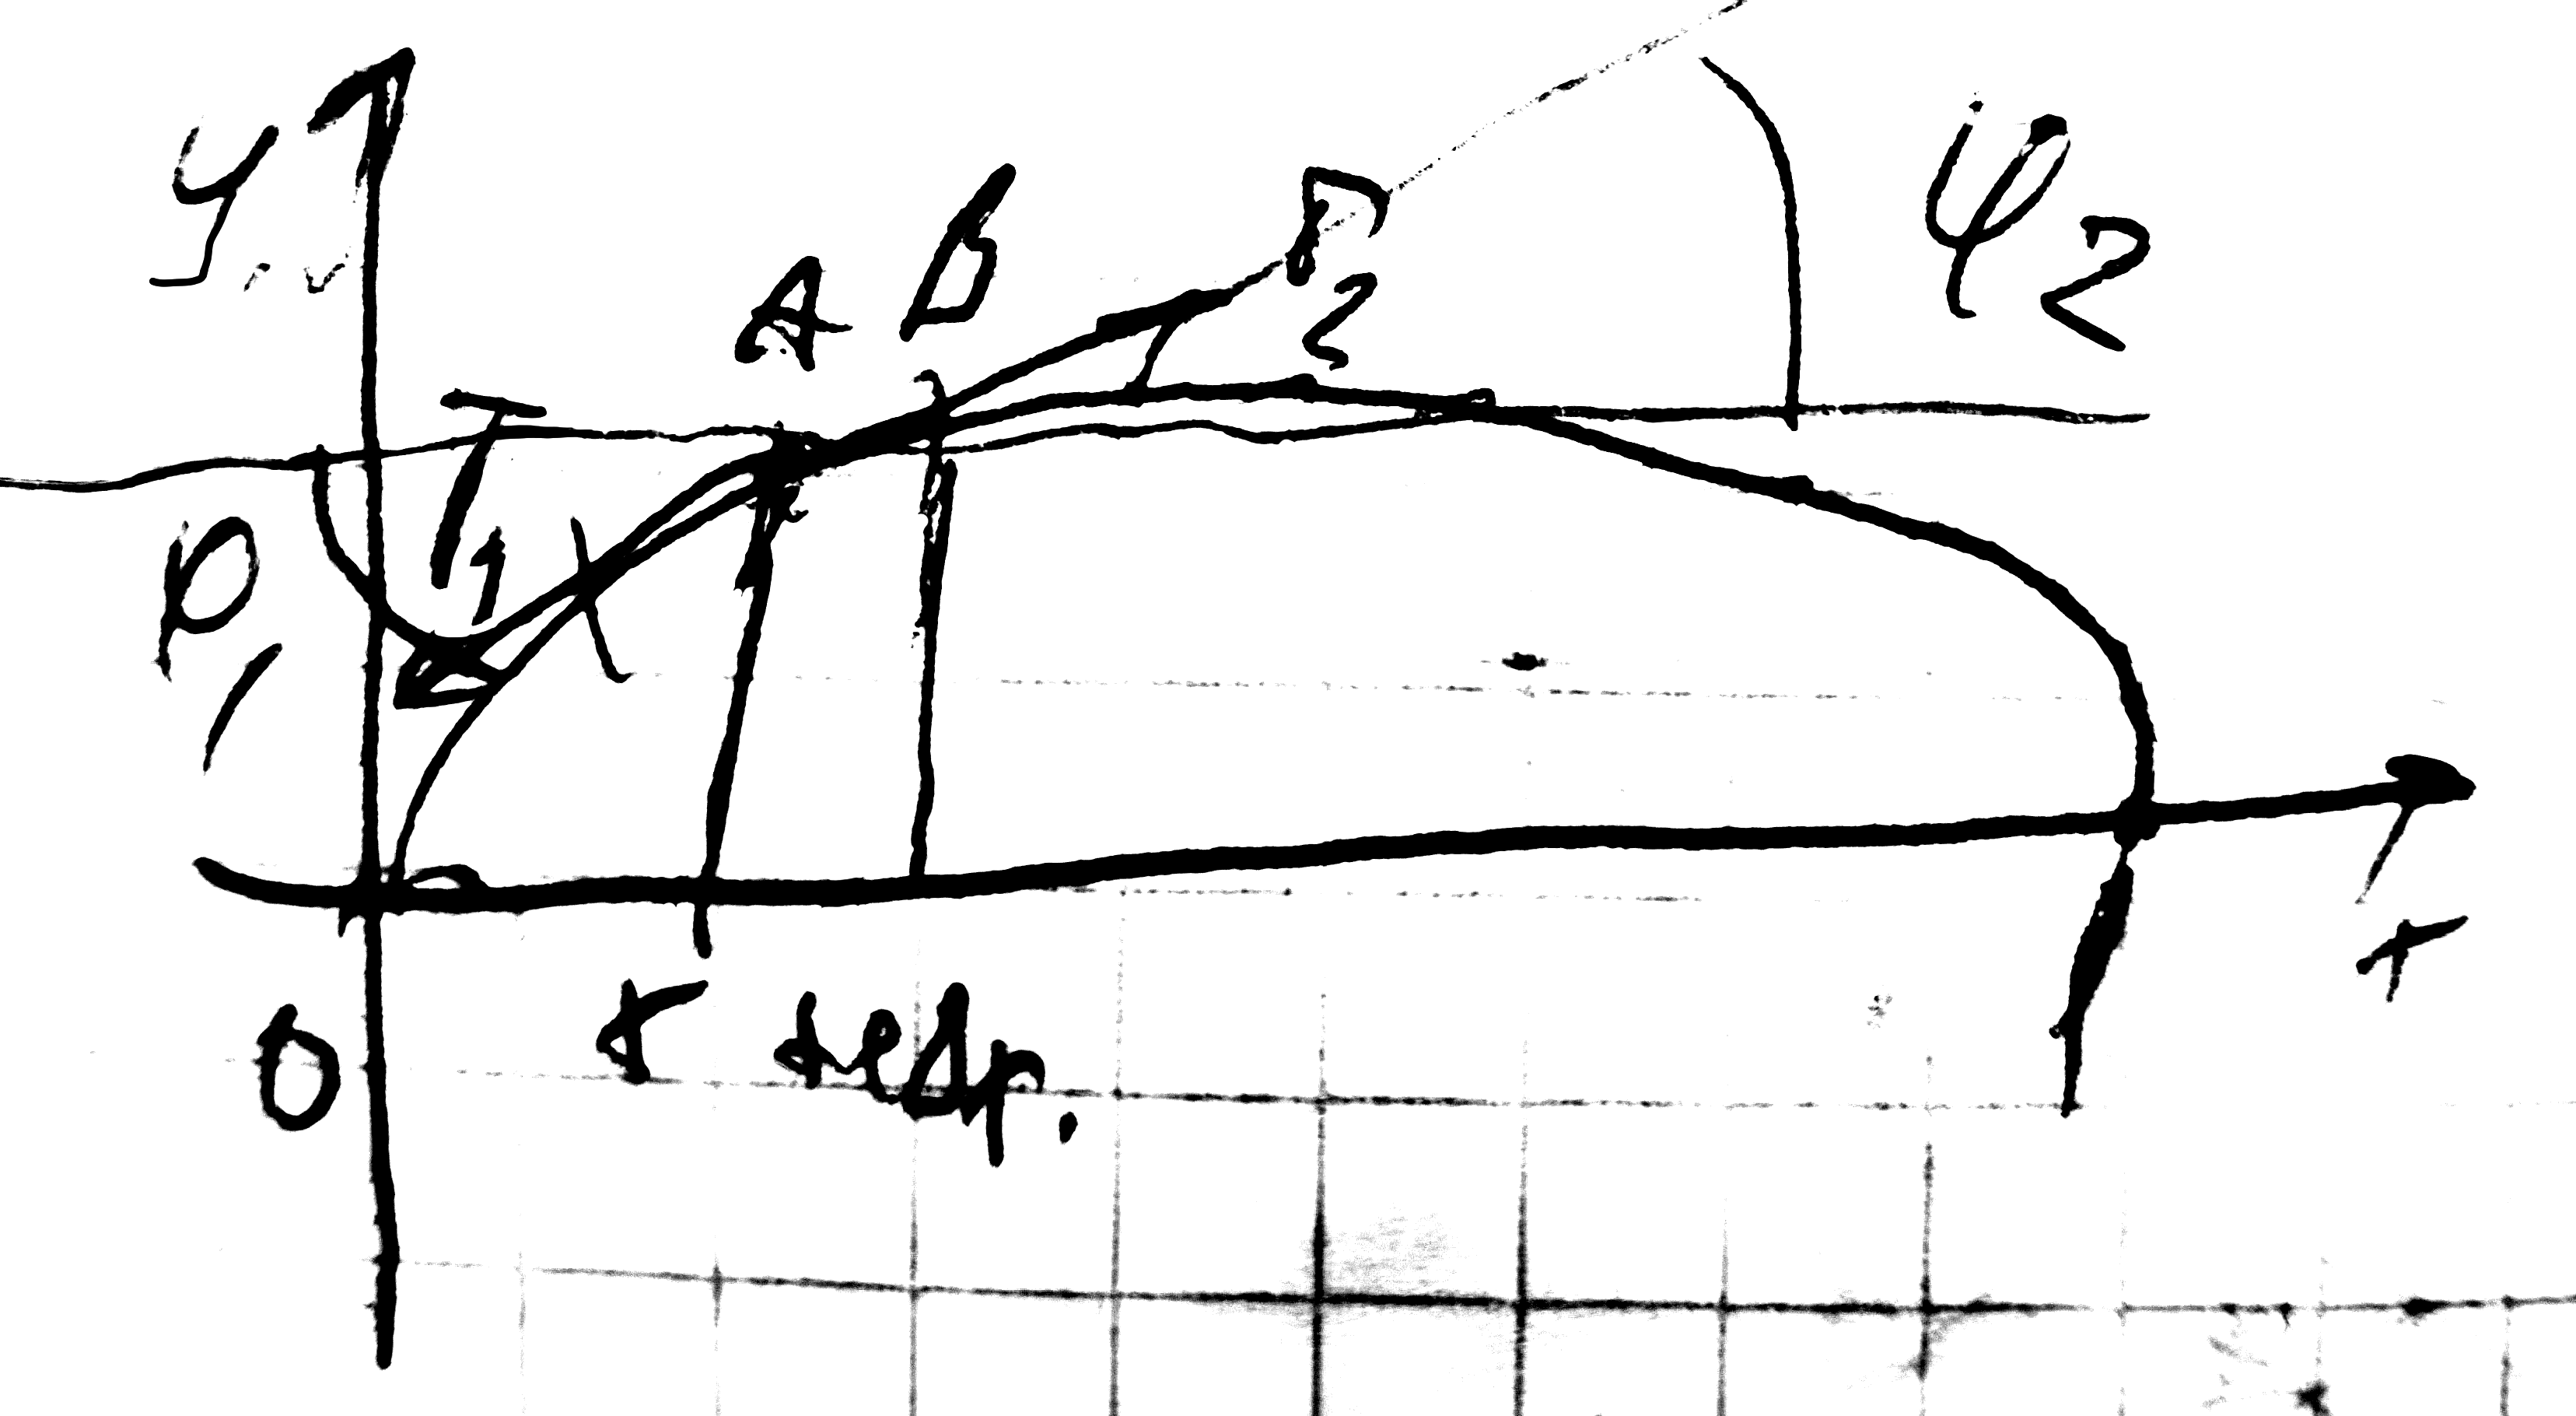
\includegraphics[width=\textwidth]{1}
\end{figure}

Силой тяжести мы пренебрегаем, продольное движение отсутствует, а остаются только две силы натяжения нити $T_1, T_2$. Спроецируем их на оси:
\[
		Ox: 0=-T_1 \cos \varphi_1 + T_2 \cos \varphi_2
\]
\[
	\begin{aligned}
		\sin \varphi = \frac{\frac{\partial u}{\partial x}}{\sqrt{1 + \left( \frac{\partial u}{\partial x}\right)^2}} \approx \frac{\partial u}{\partial x}\\
	\cos \varphi = \frac{1}{\sqrt{1 + \left( \frac{\partial u}{\partial x}\right)^2}} \approx 1
\end{aligned}
\]
Отсюда получается, что $T_1 \approx T_2 =: T$. Спроецируем на $Ou:$
\[
	\begin{aligned}
	ma = T \sin\varphi_2 - T \sin \varphi_1 \\
	ma = T \left(\left. \frac{\partial u}{\partial x}\right|_{x = x+\Delta x} - \left. \frac{\partial u}{\partial x}\right|_{x=x} \right)
\end{aligned}
\]
Массу можно представить в виде $m = l \cdot \rho$, где $l$ - длина, $\rho=const$ - линейная плотность, тогда
\[
	l = \int\limits_{AB} ds = \int\limits_x^{x+\Delta x} \sqrt{1 + \left( \frac{\partial u}{\partial x}\right)^2}dx \approx \Delta x
\]
Отсюда
\[
	\begin{aligned}
	m = \rho \cdot \Delta x \\
	\rho \Delta x \frac{\partial^2 u}{\partial t^2} = T \left(\left. \frac{\partial u}{\partial x}\right|_{x = x+\Delta x} - \left. \frac{\partial u}{\partial x}\right|_{x=x} \right) \\
			\rho \frac{\partial^2u}{\partial t^2} = T \frac{\partial^2 u}{\partial x^2} \\
			\frac{\partial^2 u}{\partial t^2} = a^2 \frac{\partial^2 u}{\partial x^2}
		\end{aligned}
\]
Уравнения в частных производных отличаются от обыкновенных дифференциальных уравнений тем, что в обыкновенных диффурах конечное число степеней свободы, а в уравнениях в частной производной - бесконечно много.
\section{Решение уравнения струны}
\[
	u_{tt} = a^2 u_{xx}
\]
Кроме того, есть граничные условия
\[
	\begin{aligned}
		u(0,t)=0 \\
		u(l,t)=0 
	\end{aligned} ~ \forall t
\]
и начальные
\[
	\begin{aligned}
		u(x,0) = \varphi(x) \\
		u_t(x,0) = \psi(x)
	\end{aligned} ~ x \in [0,l]
\]
Решение Эйлера получается через замену:
\[
	\left\{
	\begin{aligned}
		\xi = at + x \\
		\eta = -at + x
	\end{aligned}
	\right.
\]
решение выражается через $u_{\xi \eta}=0, u=G(\xi) + F(\eta)$.

Решение Даламбера -- ищем стоячие волны $F(x)$, такие, что 
\[
	u(x,t) = \cos \left(\omega t + \chi\right) F(x)
\] являются решением уравнения струны.

Подставим в уравнение:
\[
	\begin{aligned}
	u_{tt}(x,t) = - \omega^2 \cos (\omega t + \chi) F(x)  \\
	u_{xx}(x,t) = \cos (\omega t + \chi) F''(x) \\
	-\omega^2 \cos(\omega t + \chi) F(x) = a^2 \cos(\omega t + \chi) F''(x) \\
	F''(x) + \frac{\omega^2}{a^2} F(x) = 0 \\
	u(0,t) = \cos(\omega t + \chi) F(0) = 0 ~ \forall t \implies F(0) = 0 \\
	F(l) = 0
\end{aligned}
\]
Решаем диффур второго порядка и получаем решение:
\[
	\begin{aligned}
	F(x) = c \sin \frac{\omega}{a} x \\
	F(l) = c \sin \frac{\omega}{a} l = 0 \implies \frac{\omega}{a}l = \pi k, k \in \mathbb{N} \\
	\omega_k = \frac{a \pi}{l} k \\
	F_k (x) = C \sin \left(\frac{\pi k}{l} x\right)
\end{aligned}
\]
Из этого можно получить метод Фурье. Если сложить все $F_k$ в одну функцию, то получится
\[
	u(x,t) = \sum_{k=1}^\infty C_k \cos(\omega_k t+\chi_k)\sin \left( \frac{\pi k}{l} x\right) = \dots
\]
т.е. ряд Фурье. Это будет общее решение.
\[
	\dots = \sum_{k=1}^\infty \left( A_k \cos (\omega_k t) \sin \left( \frac{\pi k}{l} x\right) + B_k \sin (\omega_k t) \sin \left( \frac{\pi k}{l} x\right)\right)
\]
Неизвестными будут $A_k, B_k$. Они подбираются так, чтобы удовлетворить начальным условиям.

Посчитаем полную энергию струны.

\begin{figure}[H]
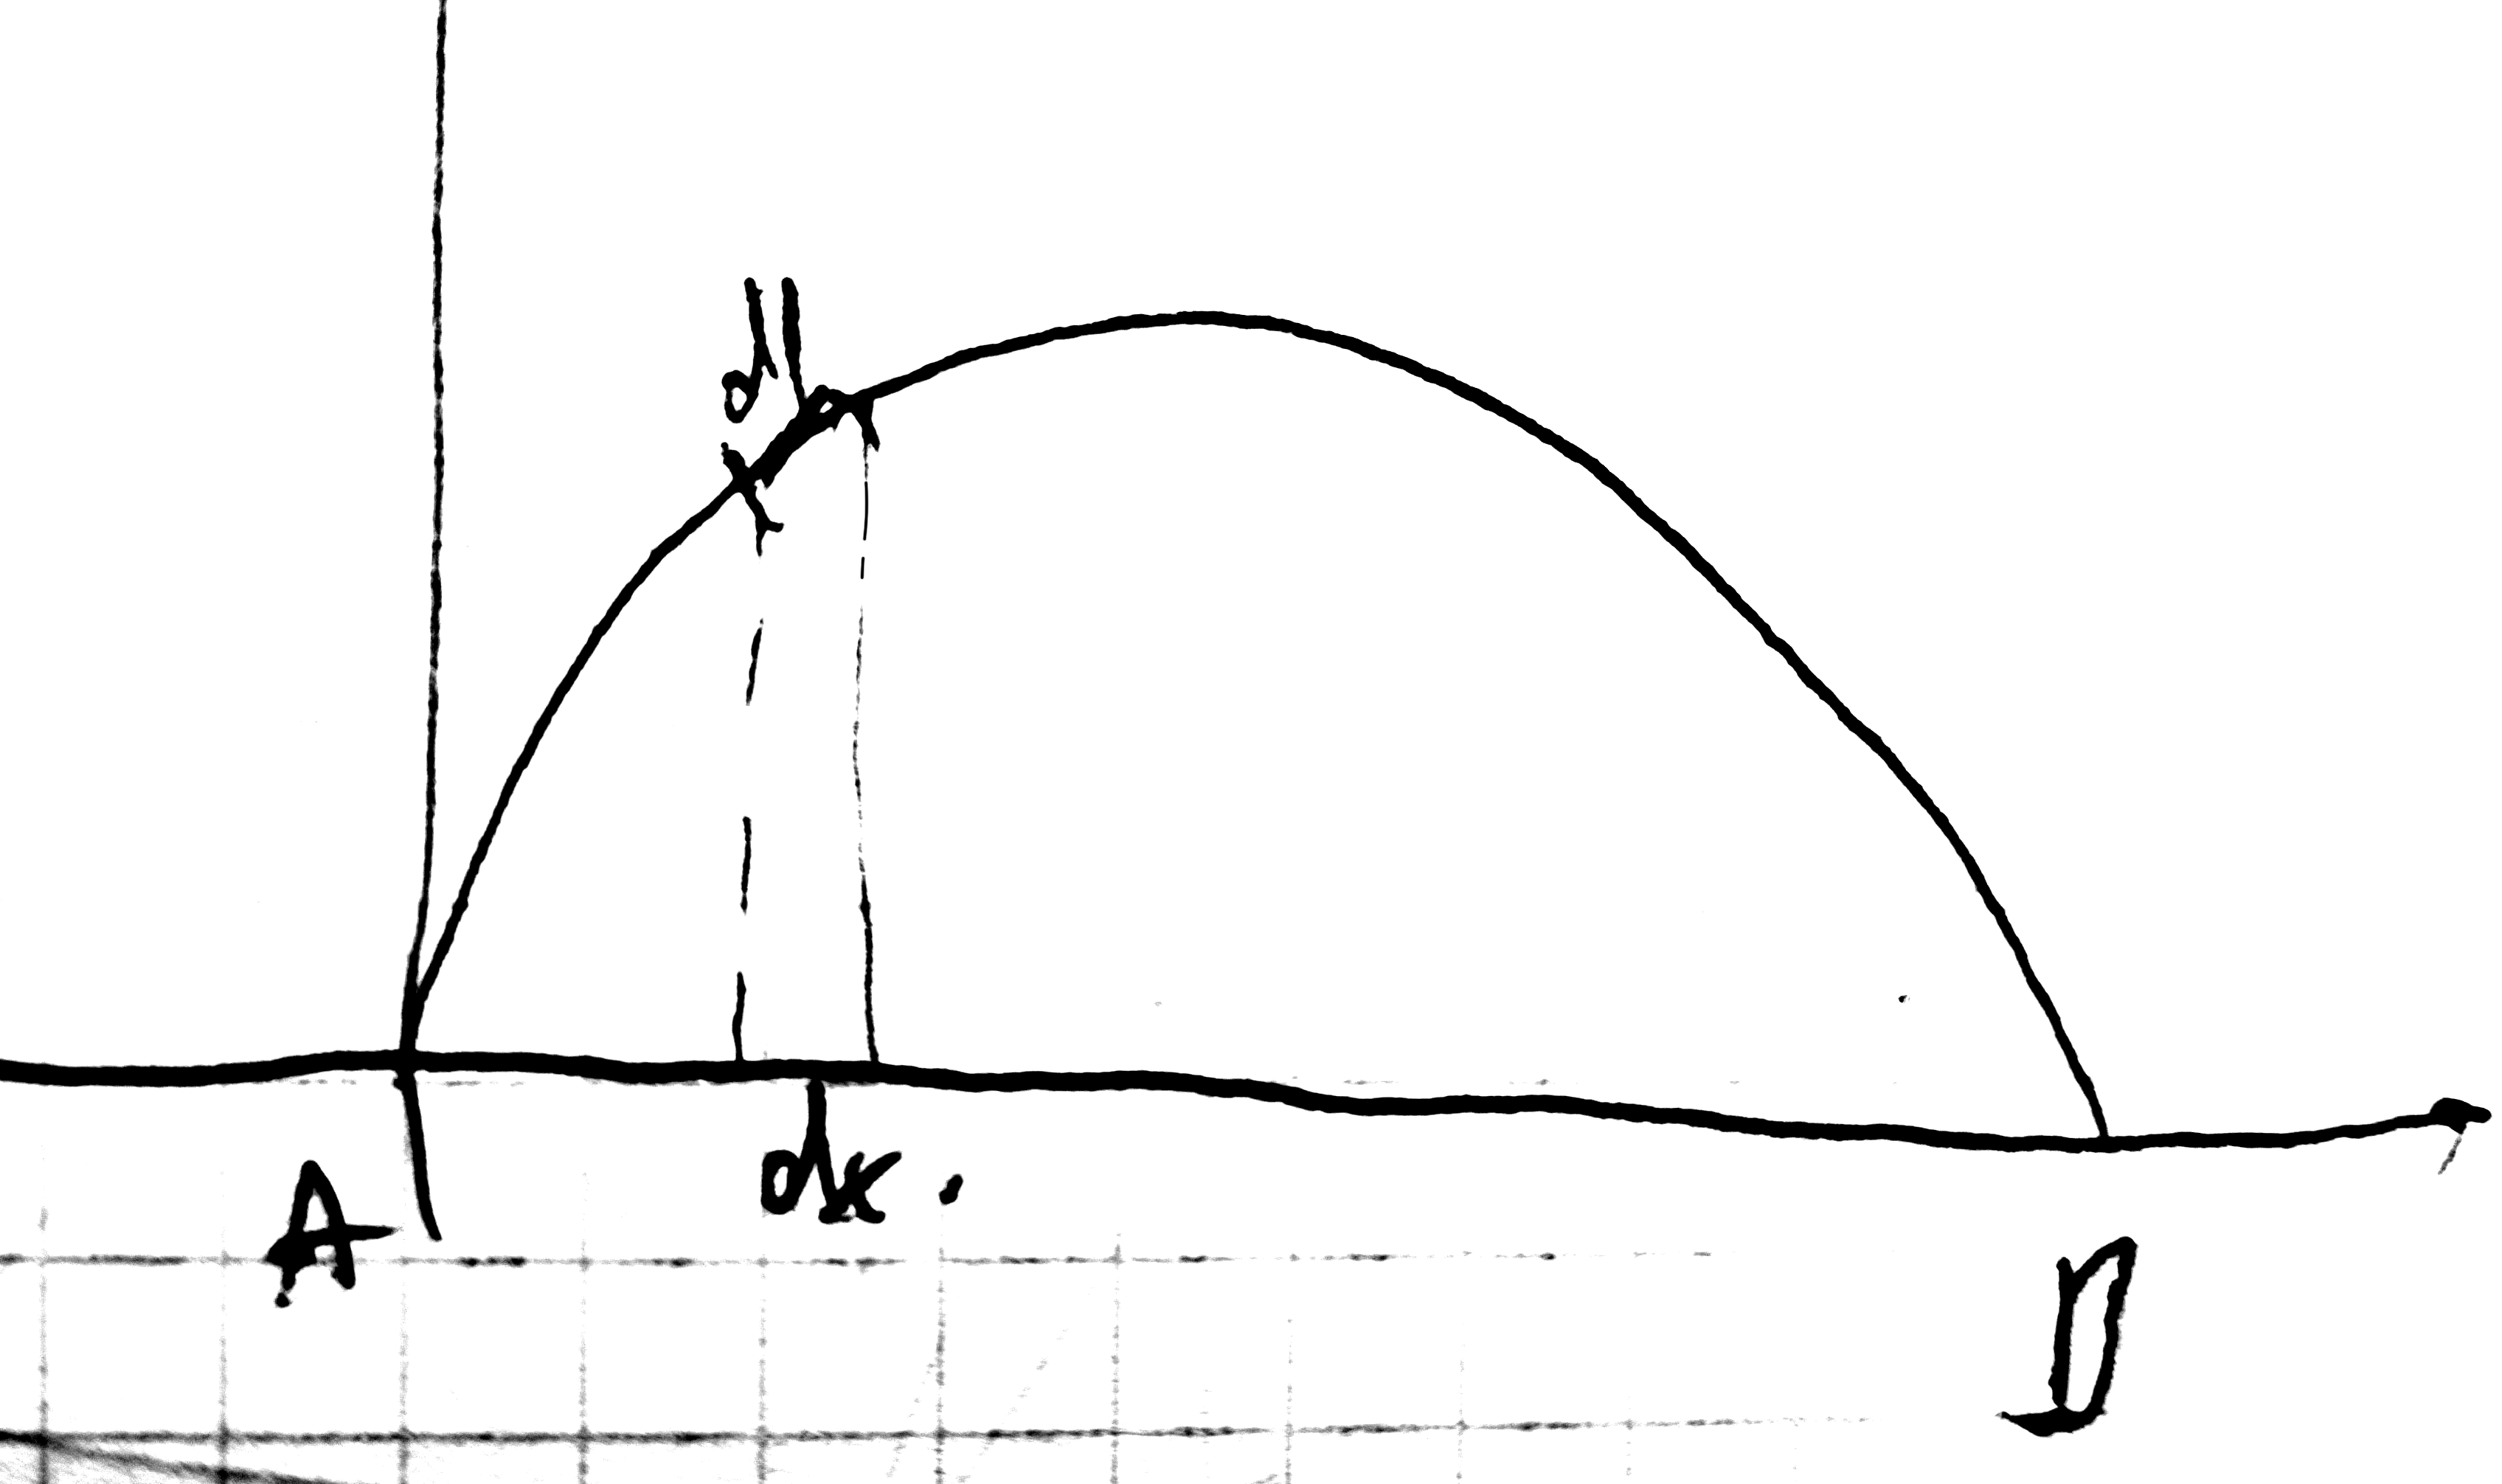
\includegraphics[width=\textwidth]{2}
\end{figure}
\[
	\begin{aligned}
	E = E_\text{К}+E_\text{П} \\
	\mathrm{d}E_\text{К} = \frac{\mathrm{d}m \cdot u_t^2}{2} = \frac{\rho \mathrm{d}l u_t^2}{2} \\
	E_\text{К} = \int\limits_{AB} \frac{\rho \mathrm{d}l \cdot u_t^2}{2} = \int\limits_0^l \frac{\rho u_t^2}{2} \sqrt{1+u_x^2} \mathrm{d}x = \\
	= \frac{\rho}{2} \int\limits_0^l u_t^2 \sqrt{1+u_x^2} \mathrm{d}x \approx \frac{\rho}{2} \int\limits_0^l u_t^2 \mathrm{d}x \\
	\mathrm{d} E_\text{П} = T \underbrace{\left( \mathrm{d}l-\mathrm{d}x\right)}_{\text{удлинение струны}} \\
	E_\text{П} = \int\limits_{AB} T(\mathrm{d}l-\mathrm{d}x) = T \int\limits_0^l \left( \sqrt{1+u_x^2} - 1\right)\mathrm{d}x \approx \\
	\approx \frac{T}{2} \int\limits_0^l u_x^2 \mathrm{d}x \\
	E = E_\text{К} + E_\text{П} \approx \frac{\rho}{2} \int\limits_0^l u_t^2 dx + \frac{T}{2} \int\limits_0^l u_x^2 \mathrm{d}x = \dots\\
	a^2 = \frac{T}{\rho} \implies \\
	\dots = \frac{\rho}{2} \int\limits_0^l \left[ u_t^2 + a^2 u_x^2\right] \mathrm{d}x
\end{aligned}
\]
Рассмотрим тогда функцию вида
\[
	u(x,t) = \cos \left( \omega_k t + \varphi\right) \sin \left( \frac{\omega_k}{a} x\right)
\]
Для неё
\[
	\begin{aligned}
	u_t^2 + a^2 u_x^2 = \omega_k^2 \sin^2 \left( \omega_k t + \varphi\right) \sin^2 \left( \frac{\omega_k}{a} x\right) + \omega_k^2 \cos^2 \left( \omega_k t + \varphi\right)\cos^2 \left( \frac{\omega_k}{a} x\right) = \\
	= \frac{\omega_k^2}{2} + \dots \cos \left( \frac{2 \omega_k}{a} x\right) \\
	E = \frac{\rho}{2} \cdot \frac{\omega_k^2} l = \frac{\rho}{4} \frac{\pi^2 k^2 a^2}{l}
\end{aligned}
\]
Отсюда получается, что чтобы заставить струну колебаться с $k$-й гармоникой, надо $k^2$ энергии.
\section{Метод Фурье для уравнения свободных колебаний струны}
Рассмотрим решение задачи о колебании однородной струны, закреплённой на концах. Эта задача сводится к решению уравнения
\[
	\frac{\partial^2 u}{\partial t^2} = a^2 \frac{\partial^2 u}{\partial x^2} \tag{1}
\]
при граничных условиях
\[
	\left. u\right|_{x=0} =0, \left. u\right|_{x=l}=0 \tag{2}
\]
и начальных условиях
\[
	\left. u\right|_{t=0}=f(x), \left.\frac{\partial u}{\partial t} \right|_{t=0} = F(x) ~ (0 \le x \le l) \tag{3}
\]
Будем искать частные решения (1), не равные тождественно нулю, (т.е. \textbf{нетривиальные}) в виде

\[
	u(x, t)=X(x)T(t) \tag{4}
\]
удовлетворяющим (2).

Подставив (4) в (1), получим
\[
	T''(t) X(x) = a^2 T(t) X''(x)
\]
или
\[
	\frac{T''(t)}{a^2 T(t)} = \frac{X''(x)}{X(x)} \tag{5}
\]
Т.к. левая часть (5) зависит только от $t$, а правая - только от $x$, то равенство возможно только когда $\frac{T''(t)}{a^2 T(t)}=\frac{X''(x)}{X(x)}=-\lambda$, $\lambda - const$.

Из (5) получим тогда:
\[
	T''(t) + a^2 \lambda T(t)=0 \tag{6}
\]
\[
	X''(x) + \lambda X(x) = 0 \tag{7}
\]
Чтобы найти нетривиальные решения вида (4), удовлетворяющие (2), необходимо найти решения уравнения (7), удовлетворяющие
\[
	X(0)=0, X(l)=0 \tag{8}
\]
Те $\lambda$, при которых (7)-(8) имеет нетривиальные решения, называются \textbf{собственными числами (значениями)}, а сами эти решения - \textbf{собственными функциями}

Найдем собственные функции и значения (7)-(8). Рассмотрим три случая $\lambda<0, \lambda=0, \lambda>0$.
\begin{enumerate}
	\item{
			$\lambda<0$. Общее решение (7) имеет вид
			\[
				X(x) = C_1 e^{\sqrt{-\lambda}x} + C_2 e^{-\sqrt{-\lambda}x}
			\]
			Удовлетворяя граничным условиям (8), получим
			\[
				C_1 + C_2 = 0, C_1 e^{\sqrt{-\lambda} l}+C_2 e^{-\sqrt{-\lambda}l}=0 \tag{9}
			\]
			Так как определитель системы (9) отличен от нуля, то $C_1=0$ и $C_2=0 \implies X(x)\equiv 0$. 
	}
	\item{
			При $\lambda=0$ общее решение (7) имеет вид
			\[
				X(x) = C_1 + C_2 x
			\]
			Граничные условия (8) дают
			\[
				C_1 = 0, C_1 + C_2 l = 0,
			\]
			поэтому $C_1=C_2=0 \implies X(x)\equiv0.$
	}
	\item{
			При $\lambda > 0$ общее решение (7) имеет вид
			\[
				X(x) = C_1 \cos \sqrt{\lambda} x + C_2 \sin \sqrt{\lambda} x.
			\]
			Удовлетворяя (8), получим
			\[
				C_1 \cdot 1 + C_2 \cdot 0 = 0, ~ C_1 \cos \sqrt{\lambda} l + C_2 \sin \sqrt{\lambda} l = 0.
			\]
			Из первого уравнения $C_1 = 0$, из второго $C_2 \sin \sqrt{\lambda} l = 0$. Мы должны считать $C_2 \ne 0$, ибо в противном случае $X(x) \equiv 0$. Поэтому $\sin \sqrt{\lambda} l = 0$, то есть $\sqrt{\lambda} = \frac{k \pi}{l}, k \in \mathbb{Z}$.

			Нетривиальные решения (7)-(8) возможны при
			\[
				\lambda_k = \left( \frac{k \pi}{l} \right)^2 ~ (k \in \mathbb{N})
			\]

			Этим $\lambda_k$ соответствуют собственные функции
			\[
				X_k (x) = \sin \frac{k \pi x}{l},
			\]
			определяемые с точностью до постоянного множителя $C$. Положим $C=1$.

			Разные $k$, отличающиеся только знаком, дают собственные функции, отличающиеся лишь постоянным множителем. Поэтому достаточно рассматривать $k \in \mathbb{N}$.

			При $\lambda = \lambda_k$ общее решение уравнения (6) имеет вид
			\[
				T_k (t) = a_k \cos \frac{k \pi at}{l} + b_k \sin \frac{k \pi at}{l}
			\]
			$a_k, b_k - \mathrm{const}$.

			Таким образом, функции
			\[
				u_k (x, t) = X_k (x) T_k (t) = \left( a_k \cos \frac{k \pi at}{l} + b_k \sin \frac{k \pi at}{l} \right) \sin \frac{k \pi x}{l}
			\]
			удовлетворяют (1) и граничным условиям (2) $\forall a_k, b_k$.

			(1) линейно и однородно, поэтому конечная сумма таких решений также будет решением. Аналогично для ряда
			\[
				u(x, t) = \sum_{k=1}^\infty \left( a_k \cos \frac{k \pi at}{l} + b_k \sin \frac{k \pi at}{l} \right) \sin \frac{k \pi x}{l}, \tag{10}
			\]
			если он сходится и его можно дважды почленно дифференцировать по $x$ и $t$. Т.к. каждое слагаемое в (10) удовлетворяет граничным условиям (2), то (2) будет удовлетворять и суммя ряда $u(x, t)$. Остается определить $a_k, b_k$ так, чтобы удовлетворить условиям (3).

			Продифференцируем (10) по $t$:
			\[
				\frac{\partial u}{\partial t} = \sum_{k=1}^\infty \frac{k \pi a}{l} \left( -a_k \sin \frac{k \pi at}{l} + b_k \cos \frac{k \pi at}{l} \right) \sin \frac{k \pi x}{l} \tag{11}
			\]
			Полагая в (10) и (11) $t=0$, в силу (3), получим:
			\[
				\begin{aligned}
					f(x) = \sum_{k=1}^\infty a_k \sin \frac{k \pi x}{l} \\
					F(x) = \sum_{k=1}^\infty \frac{k \pi a}{l} b_k \sin \frac{k \pi x}{l}
				\end{aligned}
				\tag{12}
			\]
			Формулы (12) представляют разложение $f(x), F(x)$ в ряд Фурье по синусам в интервале $(0, l)$. Коэффициенты разложений (12) выписываются по известным формулам:
			\[
				\begin{aligned}
					a_k = \frac{2}{l} \int\limits_0^l f(x) \sin \frac{k \pi x}{l} dx \\
					b_k = \frac{2}{k \pi a} \int\limits_0^l F(x) \sin \frac{k \pi x}{l} dx
				\end{aligned}
				\tag{13}
			\]
			Таким образом, решение задачи (1)-(3) даётся рядом (10), где $a_k, b_k$ определяются формулами (13).
	}
\end{enumerate}
\subsection{Теорема}
Если $f(x)$ на отрезке $[0, l]$ дважды непрерывно дифференцируема, имеет кусочно-непрерывную третью производную и удовлетворяет условиям
\[
	f(0) = f(l) = 0, ~ f''(0) = f''(l) = 0, \tag{14}
\]
а $F(x)$ непрерывно дифференцируема, имеет кусочно-непрерывную вторую производную и удовлетворяет условиям
\[
	F(0) = F(l) = 0, \tag{15}
\]
то функция $u(x, t)$, определяемая рядом (10), имеет непрерывные производные второго порядка и удовлетворяет (1)-(3). При этом возможно почленное дифференцирование (10) по $x$ и $t$ два раза, а полученные ряды будут абсолютно и равномерно сходящимися при $0 \le x \le l$ и $\forall t$.

\textbf{Доказательство}

Интегрируя по частям (13) и принимая во внимание (14)-(15), получим
\[
	\begin{aligned}
		a_k = - \left( \frac{l}{\pi} \right)^3 \frac{b_k^{(3)}}{k^3} \\
		b_k = - \left( \frac{l}{\pi} \right)^3 \frac{a_k^{(2)}}{k^3}
	\end{aligned}
	\tag{16}
\]
где
\[
	\begin{aligned}
		b_k^{(3)} = \frac{2}{l} \int\limits_0^l f'''(x) \cos \frac{k \pi x}{l} dx \\
		a_k^{(2)} = \frac{2}{l} \int\limits_0^l \frac{F''(x)}{a} \sin \frac{k \pi x}{l} dx
	\end{aligned}
	\tag{17}
\]
Из теории тригонометрических рядов известно, что ряды
\[
	\sum_{k=1}^\infty \frac{\left| a_k^{(2)} \right|}{k}, ~ \sum_{k=1}^\infty \frac{\left| b_k^{(3)} \right|}{k} \tag{18}
\]
сходятся. Подставив (16) в (10), получим
\[
	u(x, t) = - \left( \frac{l}{\pi} \right)^3 \sum_{k=1}^\infty \frac{1}{k^3} \left( b_k^{(3)} \cos \frac{k \pi at}{l} + a_k^{(2)} \sin \frac{k \pi at}{l} \right) \sin \frac{k \pi x}{l} \tag{19}
\]
Этот ряд мажорируется рядом
\[
	\left( \frac{l}{\pi} \right)^3 \sum_{k=1}^\infty \frac{1}{k^3} \left( \left| b_k^{(3)} \right| + \left| a_k^{(2)} \right| \right),
\]
который сходится. Следовательно, (10) сходится абсолютно и равномерно. Из (18), (10) можно дважды почленно дифференцировать по $x$ и $t$.

$\square$.

Если $f(x)$ и $F(x)$ не удовлетворяют условиям теоремы, то может не существовать дважды непрерывно дифференцируемого решения смешанной задачи (1)-(3). Однако, если $f(x)$ - непрерывно дифференцируемая функция, для которой $f(0) = f(l) = 0$, а $F(x)$ - непрерывная функция, для которой $F(0) = F(l) = 0$, то (10) равномерно сходится при $0 \le x \le l$ и любом $t$ и определяет непрерывную $u(x, t)$.

Будем называть \textbf{обобщённым решением} уравнения (1) при условиях (2)-(3) функцию $u(x, t)$, являющуюся пределом равномерно сходящейся последовательности $u_n (x,t)$ решений уравнения (1), удовлетворяющих (2)-(3), где $f_n(x), F_n(x)$ - последовательности функций, удовлетворяющих условиям теоремы выше и таких, что
\[
	\lim\limits_{n \to \infty} \int\limits_0^l \left[ f(x) - f_n (x) \right]^2 dx = \lim\limits_{n \to +\infty} \int\limits_0^l \left[ F(x) - F_n (x) \right]^2 dx = 0.
\]
При этих предположениях на $f(x), F(x)$, частные суммы ряда (10) образуют последовательность $u_n(x, t)$, удовлетворяющую условиям, следовательно обобщенное решение существует и ряд (10) является таким решением.

Нетрудно показать, что обобщённое решение смешанной задачи (1)-(3) единственно.

Возвратимся к найденному решению (10) задачи (1)-(3).

Ввведём обозначения
\[
	a_k = A_k \sin \varphi_k, ~ b_k = A_k \cos \varphi_k
\]
и запишем это решение в виде
\[
	u(x, t) = \sum_{k=1}^\infty A_k \sin \frac{k \pi x}{l} \sin \left( \frac{k \pi at}{l} + \varphi_k \right) \tag{20}
\]
Каждый член этого ряда представляет собой стоячую волну, при которой точки $x$ струны совершают гармоническое колебательной движение с амплитудой $A_k \sin \frac{k \pi x}{l}$, частотой $\omega_k = \frac{k \pi a}{l}$ и фазой $\varphi_k$.

\textit{уфф}

Звуки можно классифицировать на музыкальные и немузыкальные - первые называются \textbf{нотами}, вторые \textbf{шумами}. Музыкальные звуки естественным образом располагаются в определённом порядке соответственно высоте -- качеству, которое до известной степени может оценивать каждый. Те ноты, которые ухо не может различать по высоте, далее называются \textbf{тонами}.

При колебании струна издаёт звук, высота которого зависит от частоты колебаний; частота основного (самого низкого) тона выражается формулой $\omega_1 = \frac{\pi}{l} \sqrt{\frac{T_0}{\rho}}$. Тона, соответствующие более высоким частотам, чем основная, называются \textbf{обертонами}. Обертоны, частоты которых являются кратными основной частоте, называются \textbf{гармониками}. Первой гармоникой будем считать основной тон, второй гармоникой - тон с частотой $\omega_2 = 2 \omega_1$ и т.д.

\textit{Вроде $T_0$ - натяжение струны, $\rho$ - линейная плотность}

Решение (20) складывается из отдельных гармоник. Амплитуды их, а потому и влияния их на звук, издаваемый струной, обыкновенно быстро убывают при увеличении номера гармоники и всё их действие сводится к созданию тембра звука, различного для разных музыкальных инструментов и объясняемого именно наличием этих гармоник.

Существует очень мало колебательных систем с гармоническими обертонами, но эти немногие системы являются основными для построения почти всех музыкальных инструментов. Это следует из того, что звук с гармоническими обертонами кажется особенно приятным в музыкальном отношении.

В точках
\[
	x = 0, \frac{l}{k}, \frac{2l}{k}, \dots, \frac{k-1}{k} l, l
\]
амплитуда колебаний $k$-й гармоники обращается в нуль, ибо в этих точках $\sin \frac{k \pi x}{l}=0$. Эти точки называются \textbf{узлами} $k$-й гармоники. Напротив, в точках
\[
	x = \frac{l}{2k}, \frac{3l}{2k}, \dots, \frac{(2k-1)}{2k} l,
\]
называемых пучностями, амплитуда $k$-й гармоники достигает наибольшей величины, т.к. $\sin \frac{k \pi x}{l}$ там имет максимальное абсолютное значение.

Если мы прижмём колеблющуюся струну точно в середине, то есть в пучности её основного тона, то обратятся в нуль амплитуды не только этого тона, но и всех других, имеющих пучность в этой точке, то есть нечетнх гармоник. Напротив, на чётные гармоники, которые имеют узел в прижатой точке, это влиять не будет. Таким образом, остаются только четыре гармоники. Самой низкой частотой будет $\omega_2 = \frac{2 \pi}{l} \sqrt{\frac{T_0}{\rho}}$, и струна будет издавать не своё основной звук, а его октаву, то есть звук с числом колебаний в секунду вдвое большим.
